\documentclass[
  oneside,
  fullwidthstop=false,
  fontset=fandol,
  times=false,
  minted=true,
]{tongjithesis}

%%%%%%%%%%%%%%%%%%%%%%%%%%%%%%%%%%%%%%%%%%%%%%%%%%%%%%%%
% 引用文献的设置:请选择以下两种方式之一(A或B)
% Citation setup: Please choose ONE method (A or B)
%%%%%%%%%%%%%%%%%%%%%%%%%%%%%%%%%%%%%%%%%%%%%%%%%%%%%%%%

%%%%%%%%%%%%%%%%%%%%%%%%%%%%%%%%%%%%%%%%%%%%%%%%%%%%%%%%
% A. 使用 biblatex(推荐,功能更强大)
% A. Using biblatex (recommended, more powerful)
%%%%%%%%%%%%%%%%%%%%%%%%%%%%%%%%%%%%%%%%%%%%%%%%%%%%%%%%
\usepackage[
  backend=biber,      % 使用biber作为后端处理引擎
  style=gb7714-2015,  % 使用符合GB/T 7714-2015标准的引用样式
  natbib=true,        % 兼容natbib命令
]{biblatex}
\addbibresource{bib/note.bib} % 指定参考文献数据库文件

%%%%%%%%%%%%%%%%%%%%%%%%%%%%%%%%%%%%%%%%%%%%%%%%%%%%%%%%
% B. 使用 bibtex 配合 gbt7714 宏包(传统方式)
% B. Using bibtex with gbt7714 package (traditional method)
%%%%%%%%%%%%%%%%%%%%%%%%%%%%%%%%%%%%%%%%%%%%%%%%%%%%%%%%
% \usepackage[sort&compress]{gbt7714}  % 加载gbt7714宏包,支持排序和压缩引用编号
% \bibliographystyle{gbt7714-numerical} % 设置符合GB/T 7714标准的数字式引用样式
% \setlength{\bibsep}{3pt} % 设置参考文献条目之间的间距

\begin{document}

\school{计算机科学与技术学院}
\major{计算机科学与技术\quad{}计算机科学与技术\quad{}数据科学与大数据}
\student{2351570\quad{}2351579\quad{}2352976}{程浩然\quad{}樊林珂\quad{}吉镓熠}
\thesistitle{机器学习大作业一}{回归学习}
\thesistitleeng{机器学习大作业一}{回归学习}
\thesisadvisor{李\quad{}洁}
\thesisdate{\the\year}{\the\month}{\the\day} % 使用当前日期; 也可以自定义日期

\MakeCover

\cleardoublepage


\clearpage
\tableofcontents   % 放置目录
\cleardoublepage

\pagestyle{mainstyle}
\section{课程综述}

回归分析是一类重要的监督学习算法,主要用于预测连续型目标变量。其核心思想是建立特征变量与目标变量之间的映射关系,广泛应用于经济预测、医学研究、工程控制等领域。
\subsection{课题简介}
在机器学习研究领域中,传统回归算法(如最小二乘线性回归、岭回归、Lasso、Elastic Net 等)以参数可解释性强、样本效率高与训练稳定为主要优势,被广泛用于连续变量预测与因果线索探索。其核心思想是基于明确的函数假设与正则化约束,最小化经验风险并抑制过拟合。本项目基于Ridge Net构建回归模型,采用K折交叉验证 进行选参,并以MSE/MAE在独立测试集评估性能。
\subsection{课题目标}
课题的目标为对于目标数据集"Boston House Prices”,搭建相应的传统机器学习回归模型,完成用房屋的多维属性预测最终售价,并能取得较优的性能。整个实验课题包含数据准备、数据预处理、模型搭建、模型训练、模型优化、模型检测、实验总结等过程。
\subsection{线性回归的历史发展}

线性回归作为最古老、最基础的回归方法,其历史可以追溯到19世纪初:

\begin{itemize}
    \item \textbf{1805年}:法国数学家勒让德(Adrien-Marie Legendre)首次发表最小二乘法
    \item \textbf{1809年}:德国数学家高斯(Carl Friedrich Gauss)独立提出并完善了最小二乘理论
    \item \textbf{1885年}:英国统计学家高尔顿(Francis Galton)在研究遗传问题时首次使用"回归"一词
    \item \textbf{20世纪}:费希尔(Ronald Fisher)等统计学家建立了线性回归的现代理论基础
\end{itemize}

线性回归的发展历程体现了从数学理论到实际应用的完整链条,至今仍在机器学习和统计学中占据重要地位。

\subsection{常见回归算法}

\begin{itemize}
    \item \textbf{线性回归}:通过线性函数$y = \beta_0 + \beta_1x_1 + \cdots + \beta_nx_n + \epsilon$拟合数据,最小化残差平方和
    \item \textbf{岭回归}:在线性回归基础上加入L2正则化项$\lambda\sum_{i=1}^n\beta_i^2$,防止过拟合
    \item \textbf{Lasso回归}:使用L1正则化$\lambda\sum_{i=1}^n|\beta_i|$,能够产生稀疏解,实现特征选择
\end{itemize}

\subsection{线性回归应用实例}

线性回归在实际中有广泛的应用,以下是一些典型实例:

\textbf{房价预测}:
\begin{itemize}
    \item 使用房屋面积、卧室数量、地理位置等特征预测房价
    \item 模型形式:$\text{价格} = \beta_0 + \beta_1\times\text{面积} + \beta_2\times\text{卧室数} + \cdots$
\end{itemize}
\begin{figure}[!htb]
	\centering
	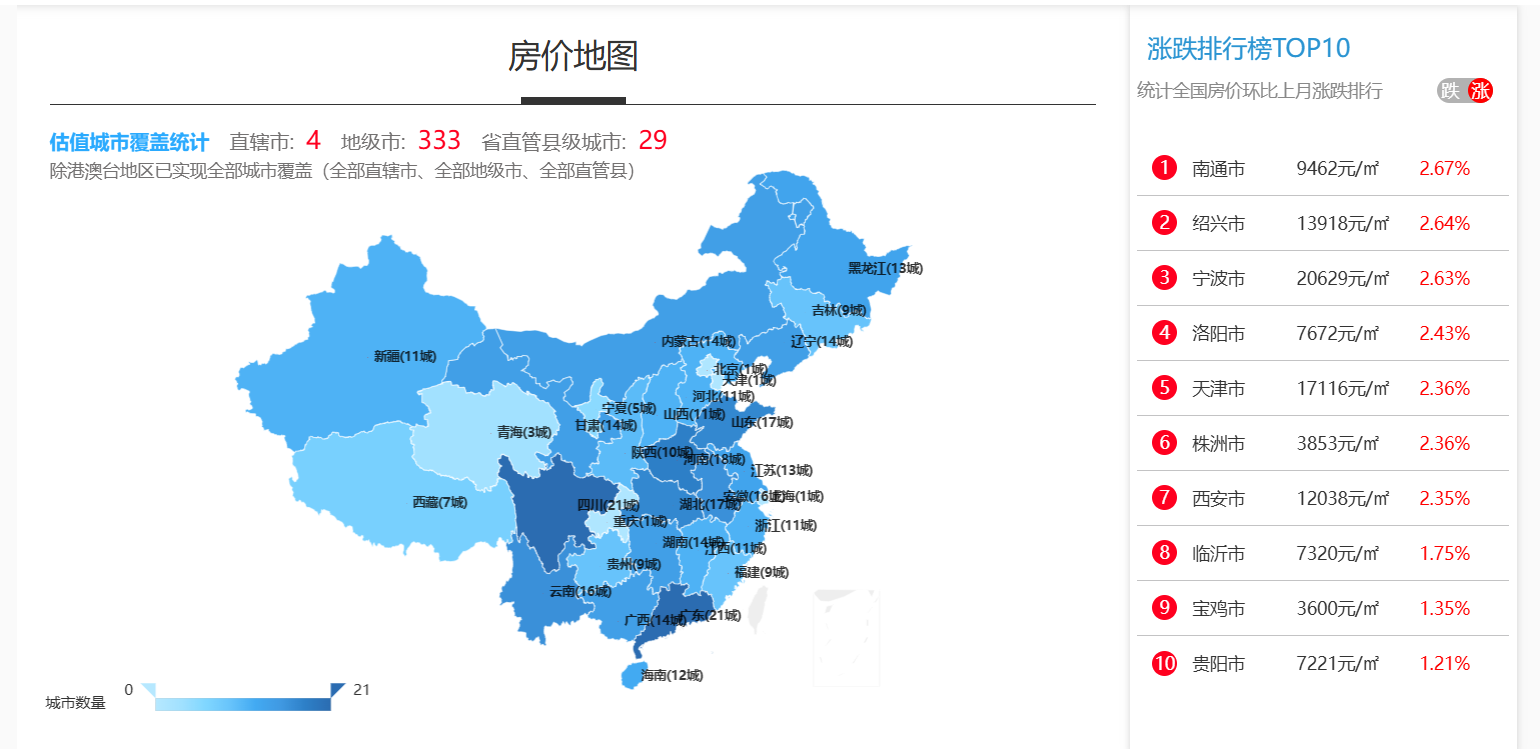
\includegraphics[width=0.70\textwidth]{./figures/house.png}
	\caption{房价地图}
\end{figure}

\textbf{医学研究}:
\begin{itemize}
    \item 基于患者年龄、体重、生活习惯等预测血压水平
    \item 分析药物剂量与治疗效果的关系
\end{itemize}

\textbf{网点数据分析}:
\begin{itemize}
    \item 分析不同平台对于电商销售额的影响。
\end{itemize}



\subsection{模型评估}

回归模型常用评估指标包括:
\begin{itemize}
    \item \textbf{均方误差(MSE)}:$\frac{1}{n}\sum_{i=1}^n(y_i - \hat{y}_i)^2$
    \item \textbf{均方根误差(RMSE)}:$\sqrt{\text{MSE}}$
    \item \textbf{平均绝对误差(MAE)}:$\frac{1}{n}\sum_{i=1}^n|y_i - \hat{y}_i|$
    \item \textbf{决定系数($R^2$)}:$1 - \frac{\sum_{i=1}^n(y_i - \hat{y}_i)^2}{\sum_{i=1}^n(y_i - \bar{y})^2}$
\end{itemize}

随着大数据时代的发展,回归分析在推荐系统、风险评估、量化投资等新兴领域继续发挥着重要作用。
\subsection{数据集选取}
基于以上的场景应用,我们选择了三个数据集用以训练自己的模型。
\subsubsection{波士顿房价数据集(Boston House Price Dataset)}
该数据集来源于\texttt{https://huggingface.co/datasets/mrseba/boston\_house\_price},是机器学习回归任务的经典基准数据集,源于1970年代美国波士顿地区住房市场普查,共包含506条样本,核心目标是通过12个输入属性预测街区的房价中位数(MEDV,单位:千美元),为房地产市场分析与区域经济研究提供数据支撑。

其12个输入属性涵盖社会、经济、环境等多维度信息,各变量详情如下表所示:

\begin{table}[!hpt]
  \caption{波士顿房价数据集特征变量详情}
  \label{tab:boston_house_features}
  \centering
  \small
  % 用p{宽度}固定列宽,总宽度控制在文本宽度内,行内自动换行
  \begin{tabular}{@{}p{0.12\textwidth}p{0.25\textwidth}p{0.18\textwidth}p{0.4\textwidth}@{}} \toprule
    \textbf{特征名称} & \textbf{变量含义} & \textbf{数据类型} & \textbf{对房价(MEDV)的影响逻辑} \\ \midrule
    CRIM & 街区人均犯罪率 & 连续型(数值) & 负相关:犯罪率越高,居住安全性越低,房价通常越低 \\
    ZN & 占地面积超过25000平方英尺的住宅用地比例 & 连续型(数值) & 正相关:大户型住宅占比高,区域居住品质偏高,房价更高 \\
    INDUS & 街区非零售商业用地比例(英亩/城镇) & 连续型(数值) & 负相关:商业用地密集可能导致居住环境嘈杂,降低居住舒适度 \\
    CHAS & 查尔斯河虚拟变量(1=临近河流,0=不临近) & 离散型(二分类) & 正相关:临水地段通常具备景观优势,房价存在“临水溢价” \\
    NOX & 一氧化氮浓度(百万分之一) & 连续型(数值) & 负相关:污染物浓度高代表环境质量差,对房价有抑制作用 \\
    RM & 每栋住宅的平均房间数 & 连续型(数值) & 强正相关:房间数越多,住宅实用面积与居住空间越大,房价显著更高 \\
    AGE & 1940年之前建成的自住单位比例 & 连续型(数值) & 负相关:房龄越长,房屋设施老化程度越高,维护成本增加,房价偏低 \\
    DIS & 到波士顿5个就业中心的加权距离 & 连续型(数值) & 负相关:距离就业中心越近,通勤便利性越强,房价越高 \\
    RAD & 到高速公路的可达性指数(指数越高可达性越好) & 连续型(数值) & 正相关:交通便利性提升居住便捷度,对房价有正向拉动 \\
    TAX & 每10000美元房产的全额财产税率 & 连续型(数值) & 负相关:税率越高,持有房产的成本越高,可能降低房价吸引力 \\
    PTRATIO & 街区师生比(学生数/教师数) & 连续型(数值) & 负相关:师生比越低(教师资源越充足),教育配套越好,房价越高 \\ \bottomrule
  \end{tabular}
\end{table}


\subsubsection{个人医疗费用数据集(Insurance Dataset)}
该数据集来源于\texttt{https://www.kaggle.com/datasets/mirichoi0218/insurance},是个性化风险预测与回归分析的典型数据集,采集自真实个人医疗保险记录,共1338条样本,核心任务是根据个人基本信息与健康状况,预测年度医疗费用(insuranceclaim),适用于保险公司保费定价、医疗成本核算场景。

数据集变量分为数值型与字符串型(需编码处理),各变量详情如下表所示:

\begin{table}[!hpt]
  \caption{个人医疗费用数据集变量详情}
  \label{tab:insurance_variables}
  \centering
  \small
  \begin{tabular}{@{}p{0.12\textwidth}p{0.2\textwidth}p{0.18\textwidth}p{0.22\textwidth}p{0.23\textwidth}@{}} \toprule
    \textbf{变量名称} & \textbf{变量含义} & \textbf{数据类型} & \textbf{取值范围/类别} & \textbf{对医疗费用的潜在影响} \\ \midrule
    age & 被保险人年龄 & 数值型(连续) & 18-64岁 & 正相关:年龄增长导致慢性病风险升高,医疗需求增加 \\
    sex & 性别 & 字符串型(分类) & "male"(男性)、"female"(女性) & 差异较小:女性可能因生育、妇科疾病产生特定费用 \\
    bmi & 体重指数(Body Mass Index) & 数值型(连续) & 15.96-53.13 & 正相关:BMI异常增加健康风险,如肥胖与糖尿病相关 \\
    children & 被保险人子女数量 & 数值型(离散) & 0-5人 & 正相关:子女数量越多,家庭整体医疗需求越高 \\
    smoker & 是否吸烟 & 字符串型(分类) & "yes"(吸烟)、"no"(不吸烟) & 强正相关:吸烟与重疾相关,医疗费用显著更高 \\
    region & 居住区域 & 字符串型(分类) & "northeast"等4个区域 & 区域差异:医疗资源、病种流行率不同导致费用差异 \\
    charges & 年度医疗费用(目标变量) & 数值型(连续) & 1121.87-63770.43美元 & - \\ \bottomrule
  \end{tabular}
\end{table}

字符串变量需针对性编码:二分类变量(sex、smoker)可采用标签编码(如male→1、female→0;yes→1、no→0),避免独热编码的特征冗余;多分类变量(region)推荐独热编码(转换为4个二进制特征),或目标编码(用区域内charges均值编码,需交叉验证防过拟合)。

\subsubsection{网店销售额预测数据集(Advertising Simple Dataset)}
该数据集来源于\texttt{https://www.kaggle.com/datasets/tohuangjia/advertising-simple-dataset},是营销效果分析与回归预测的简化数据集,共200条样本。通过记录网店不同渠道广告费用,预测同期产品销售额,适用于电商广告预算分配、营销效果评估场景。

数据集变量设计简洁,均为数值型,无需复杂的分类变量编码,各变量详情如下表所示:

\begin{table}[!hpt]
  \caption{网店销售额预测数据集变量详情}
  \label{tab:advertising_variables}
  \centering
  \small
  \begin{tabular}{@{}p{0.15\textwidth}p{0.22\textwidth}p{0.18\textwidth}p{0.25\textwidth}p{0.17\textwidth}@{}} \toprule
    \textbf{变量名称} & \textbf{变量含义} & \textbf{数据类型} & \textbf{取值范围(单位:千美元)} & \textbf{对销售额的影响逻辑} \\ \midrule
    TV & 电视广告投放费用 & 连续型 & 0.7-296.4 & 正相关:覆盖人群广,品牌曝光度高,拉动作用最强 \\
    Radio & 广播广告投放费用 & 连续型 & 0.0-49.6 & 正相关:针对特定场景,覆盖精准度较高,影响范围小于电视 \\
    Newspaper & 报纸广告投放费用 & 连续型 & 0.3-114.0 & 弱正相关/无显著相关:时效性强但留存率低,转化效果弱 \\
    Sales & 同期产品销售额(目标变量) & 连续型 & 1.6-27.0 & - \\ \bottomrule
  \end{tabular}
\end{table}
\subsubsection{代码说明}
\begin{lstlisting}[
  language=Python,         % 指定语法高亮的编程语言
  caption={下载数据集},
  label=lst:download,
  frame=single,            % 添加单线边框
  basicstyle=\small\ttfamily, % 设置字体为等宽小号字体
  numbers=left,            % 显示行号
  numberstyle=\tiny,       % 行号使用极小字体
  backgroundcolor=\color{bg}, % 设置背景色
  commentstyle=\color{commentcolor}\itshape, % 注释样式
  keywordstyle=\color{keywordcolor}\bfseries, % 关键字样式
  stringstyle=\color{stringcolor}, % 字符串样式
  breaklines=true,         % 允许自动换行
  showstringspaces=false   % 不显示字符串中的空格
]
y_label="MEDV"
_target_path="./dataset"
data_path=_target_path+"/train.csv"
title="波士顿房价数据集"
def download_dataset_boston():
	ds = load_dataset("mrseba/boston_house_price")
	ds.save_to_disk("./dataset")
	train_df = ds['train'].to_pandas()
	train_df.to_csv("./dataset/train.csv", index=False)
	print("Dataset downloaded and saved to disk.")
if __name__ == '__main__':
	download_dataset_boston()
\end{lstlisting}


\par 通过设置download.py当中的描述数据集信息的设置,可以做到对于任何一个线性回归数据集的适应。限制条件是不允许使用字符描述的列值,以及数据集必须以csv格式保存。对于每个变量说明如下:
\begin{itemize}
\item \bf{y\_label}:这个csv当中的y标签对应的列名。
\item \bf{\_target\_path}:数据集的csv文件存储的url
\item \bf{data\_path}:数据在本地存储的相对位置
\item \bf{title}:希望以什么样的名字命名这个回归图像
\end{itemize}

\par 设置好之后下载数据集 python download.py 再运行python main.py 即可开始回归



\clearpage
\section{数据准备}
\subsection{变量说明}
本实验中训练的模型表达式为:
\[
    y = \boldsymbol{\theta}_{1 \times (I+1)} \cdot \begin{bmatrix} \boldsymbol{X} \\ 1 \end{bmatrix}
\]

其中各变量定义如下:
\begin{itemize}
\item 输入向量 $\boldsymbol{X}_{I \times J} = \{x_{i}^{j}\}$:表示整体训练数据集,包含 $J$ 个样本,每个样本有 $I$ 个特征。$x_{i,j}$ 表示第 $j$ 个样本的第 $i$ 个特征值。

\item 输入向量 $\boldsymbol{x}_{I \times 1}$:表示单个样本的输入特征向量。

\item  模型参数 $\boldsymbol{\theta}_{1 \times (I+1)}$:表示待训练的系数向量,维度为 $1 \times (I+1)$(包含偏置项)。

\end{itemize}


\subsection {数据预处理过程}
\subsubsection{5折交叉分析}
\begin{lstlisting}[
  language=Python,         % 指定语法高亮的编程语言
  caption={5折交叉划分数据集},
  label=lst:pre1,
  frame=single,            % 添加单线边框
  basicstyle=\small\ttfamily, % 设置字体为等宽小号字体
  numbers=left,            % 显示行号
  numberstyle=\tiny,       % 行号使用极小字体
  backgroundcolor=\color{bg}, % 设置背景色
  commentstyle=\color{commentcolor}\itshape, % 注释样式
  keywordstyle=\color{keywordcolor}\bfseries, % 关键字样式
  stringstyle=\color{stringcolor}, % 字符串样式
  breaklines=true,         % 允许自动换行
  showstringspaces=false   % 不显示字符串中的空格
]
def createTrainAndTest(XRaw,YRaw,train_size=0.8,random_state=42):
	if random_state is not None:
		np.random.seed(random_state)
	
	n_samples = XRaw.shape[0]
	'''
	shape[0] 表示行数(即样本数量,对应代码中的n_samples);
	shape[1] 表示列数(即特征数量)。
	'''
	
	n_train = int(train_size * n_samples)
	indices = np.random.permutation(n_samples)
	
	train_indices = indices[:n_train]
	test_indices = indices[n_train:]
	
	X_train = XRaw.iloc[train_indices]
	X_test = XRaw.iloc[test_indices]
	Y_train = YRaw.iloc[train_indices]
	Y_test = YRaw.iloc[test_indices]
	return X_train,X_test,Y_train,Y_test
\end{lstlisting}
\par main.creatTrainAndTest 完成了从硬盘当中读取的$\bf X $ 数据集分割为$\bf{X_{train}} $(下称$\bf{X}$)、$\bf{X_{test}}$ 两个数据集。

\subsubsection{训练数据标准化}
训练数据的标准化通过train.preprocess\_data 完成
\par 将数据集$\bf{X}$ 求平均值:
\[
\bf{\overline{X}} =\bf{\overline{X}_{1 \times I}} = \begin{bmatrix}
\frac{\sum_{j=1}^{J} x_{1}^{j}}{J}
 \\ \frac{\sum_{j=1}^{J} x_{2}^{j}}{J}
 \\\frac{\sum_{j=1}^{J} x_{3}^{j}}{J}
\\\vdots
\\\frac{\sum_{j=1}^{J} x_{I}^{j}}{J}

\end{bmatrix} 
\]
求标准差:
\[
\boldsymbol{\sigma} = \boldsymbol{\sigma}_{I \times 1} = \begin{bmatrix}
\sqrt{\frac{\sum_{j=1}^{J} \left(x_{1}^{j} - \overline{x}_{1}\right)^2}{J}} \\
\sqrt{\frac{\sum_{j=1}^{J} \left(x_{2}^{j} - \overline{x}_{2}\right)^2}{J}} \\
\sqrt{\frac{\sum_{j=1}^{J} \left(x_{3}^{j} - \overline{x}_{3}\right)^2}{J}} \\
\vdots \\
\sqrt{\frac{\sum_{j=1}^{J} \left(x_{I}^{j} - \overline{x}_{I}\right)^2}{J}}
\end{bmatrix}
\]

于是我们可以对原数据$\bf{X}$及标准化:
\[
	\boldsymbol{X} := \begin{bmatrix}
	\frac{x_{1}^{1} - \overline{x}_{1}}{\sigma_{1}} & \frac{x_{1}^{2} - \overline{x}_{1}}{\sigma_{1}} & \cdots & \frac{x_{1}^{J} - \overline{x}_{1}}{\sigma_{1}} \\
	\frac{x_{2}^{1} - \overline{x}_{2}}{\sigma_{2}} & \frac{x_{2}^{2} - \overline{x}_{2}}{\sigma_{2}} & \cdots & \frac{x_{2}^{J} - \overline{x}_{2}}{\sigma_{2}} \\
	\vdots & \vdots & \ddots & \vdots \\
	\frac{x_{I}^{1} - \overline{x}_{I}}{\sigma_{I}} & \frac{x_{I}^{2} - \overline{x}_{I}}{\sigma_{I}} & \cdots & \frac{x_{I}^{J} - \overline{x}_{I}}{\sigma_{I}}
	\end{bmatrix}
\]

随后我们对使用过海豹运算符后的$\bf{X}$进行处理,此时的数据集是已经被标准化的。
\clearpage
\subsubsection{处理掉所有的丢失值}

这部分直接调用numpy的库函数可以完成。
\begin{lstlisting}[
  language=Python,         % 指定语法高亮的编程语言
  caption={去除nan值},
  label=lst:pre2,
  frame=single,            % 添加单线边框
  basicstyle=\small\ttfamily, % 设置字体为等宽小号字体
  numbers=left,            % 显示行号
  numberstyle=\tiny,       % 行号使用极小字体
  backgroundcolor=\color{bg}, % 设置背景色
  commentstyle=\color{commentcolor}\itshape, % 注释样式
  keywordstyle=\color{keywordcolor}\bfseries, % 关键字样式
  stringstyle=\color{stringcolor}, % 字符串样式
  breaklines=true,         % 允许自动换行
  showstringspaces=false   % 不显示字符串中的空格
]
def clear_nan(train_df):
    train_df.dropna(inplace=True)
    train_df.reset_index(drop=True, inplace=True)
    print(train_df.head())
    return train_df
\end{lstlisting}


\subsubsection{模型搭建}
\par 本节基于梯度下降法,分别构建线性回归、岭回归与Lasso回归模型,核心参数更新逻辑如下:

\paragraph{线性回归(Linear Regression)}
线性回归通过最小化预测值与真实值的平方误差更新参数,无正则化项,具体步骤为:
\begin{itemize}
\item [1] 预测值计算:
\[
\hat{y} = X \cdot \theta
\]
其中,$X$ 为输入特征矩阵(含偏置项扩展),$\theta$ 为待优化参数向量,$\hat{y}$ 为模型预测输出。

\item [2] 误差计算:
\[
e = \hat{y} - y
\]
其中,$y$ 为真实标签向量,$e$ 为预测值与真实值的误差向量。

\item [3] 梯度计算:
\[
\nabla J(\theta) = \frac{1}{m} X^T \cdot e
\]
其中,$m$ 为样本数量,$\nabla J(\theta)$ 为损失函数对参数 $\theta$ 的梯度(反映参数更新方向)。

\item [4] 参数更新:
\[
\theta = \theta - \eta \cdot \nabla J(\theta)
\]
其中,$\eta$ 为学习率(控制每次参数更新的步长)。

\item [5] 收敛条件(满足其一即可终止迭代):
\[
\|\nabla J(\theta)\| < 10^{-6} \quad \text{或} \quad \text{迭代次数} \geq \text{最大迭代次数}
\]
$\|\cdot\|$ 表示向量的L2范数,梯度范数小于 $10^{-6}$ 意味着参数更新已趋于稳定。
\end{itemize}

\paragraph{岭回归(Ridge Regression)}
岭回归在普通线性回归基础上引入\textbf{L2正则化},通过惩罚参数的平方项抑制过拟合,且不惩罚偏置项 $\theta_0$,参数更新步骤为:
\begin{itemize}
\item [1] 基础参数更新(同线性回归):
\[
\theta_{\text{temp}} = \theta - \eta \cdot \nabla J(\theta)
\]
其中,$\theta_{\text{temp}}$ 为线性回归更新后的临时参数。

\item [2] L2正则化修正(仅对非偏置项 $i \geq 1$ 生效):
\[
\theta_i = \theta_{\text{temp},i} - \eta \cdot \alpha \cdot \theta_{\text{temp},i}
\]
其中,$\alpha$ 为正则化强度($\alpha \geq 0$,值越大对参数的惩罚越强,参数越趋于平缓但不会归零),$\theta_{\text{temp},i}$ 为临时参数的第 $i$ 个分量。
\end{itemize}

\paragraph{Lasso回归(Lasso Regression)}
Lasso回归引入\textbf{L1正则化},通过惩罚参数的绝对值项实现特征选择(部分非重要参数会被压缩至0),同样不惩罚偏置项 $\theta_0$,参数更新步骤为:
\begin{itemize}
\item [1] 基础参数更新(同线性回归):
\[
\theta_{\text{temp}} = \theta - \eta \cdot \nabla J(\theta)
\]

\item [2] L1正则化修正(仅对非偏置项 $i \geq 1$ 生效):
\[
\theta_i = \theta_{\text{temp},i} - \eta \cdot \alpha \cdot \text{sign}(\theta_{\text{temp},i})
\]
其中,$\text{sign}(\cdot)$ 为符号函数(参数为正时返回1,为负时返回-1,为0时返回0),$\alpha$ 为正则化强度($\alpha$ 越大,参数被压缩至0的概率越高,特征选择效果越明显)。
\end{itemize}

\paragraph{项目支持任意梯度的植入}
想要加入新的梯度,只需要在train.py当中的对应列表加入这个回归方法的名字对应的字符串和函数指针即可。需要在这两个列表之前实现对应的函数。
\begin{lstlisting}[
  language=Python,         % 指定语法高亮的编程语言
  caption={加入时需要调整的内容},
  label=lst:pre3,
  frame=single,            % 添加单线边框
  basicstyle=\small\ttfamily, % 设置字体为等宽小号字体
  numbers=left,            % 显示行号
  numberstyle=\tiny,       % 行号使用极小字体
  backgroundcolor=\color{bg}, % 设置背景色
  commentstyle=\color{commentcolor}\itshape, % 注释样式
  keywordstyle=\color{keywordcolor}\bfseries, % 关键字样式
  stringstyle=\color{stringcolor}, % 字符串样式
  breaklines=true,         % 允许自动换行
  showstringspaces=false   % 不显示字符串中的空格
]
regression_choices=["linear_regression_train","ridge_regression_train","lasso_regression_train"]
regression_functions=[linear_regression_train,ridge_regression_train,lasso_regression_train]
\end{lstlisting}

\clearpage
\section{模型训练过程和测试过程}
为确保回归模型高效收敛并输出可靠的拟合结果,本实验构建了“预处理-训练-可视化”三位一体的完整训练流程,从数据准备到结果呈现的各环节设计如下:

\subsection{训练前的数据预处理:必要性与操作逻辑}
数据预处理是模型训练的\textbf{前置必要步骤},其有效性直接决定梯度下降算法的稳定性与收敛效率。原始输入特征矩阵$\boldsymbol{X}$中,不同特征往往存在量纲差异(例如“样本温度”特征取值范围为$[0, 100]$,“样本湿度”特征取值范围为$[0, 1]$)。若直接使用原始数据训练,会导致损失函数的梯度分布严重失衡——即使设置常规学习率(如$\eta=0.01$),也可能出现参数更新幅度过大、损失值震荡不收敛,甚至梯度爆炸等“意想不到的错误”。

因此,训练前需对$\boldsymbol{X}$执行标准化操作(基于各特征的均值$\overline{x}_i$与标准差$\sigma_i$),将所有特征映射到相近的数值区间。具体标准化公式参考前文定义:
\[
x_{i,j}^{\text{标准化}} = \frac{x_{i,j} - \overline{x}_i}{\sigma_i}
\]
其中$x_{i,j}$为原始特征值,$x_{i,j}^{\text{标准化}}$为标准化后的特征值。通过该操作,可使各特征的均值趋近于0、标准差趋近于1,为梯度下降的稳定迭代提供数据基础。

\subsection{迭代训练逻辑与收敛控制}
模型训练基于前文定义的梯度下降函数(线性回归/岭回归/Lasso回归),核心训练逻辑与终止条件设计如下:
\begin{itemize}
    \item[1] \textbf{迭代触发与参数更新}:模型启动后,每轮训练均按“预测值计算→误差求解→梯度计算→参数更新”的流程执行(对应公式$\hat{y}=X\cdot\theta$、$e=\hat{y}-y$、$\nabla J(\theta)=\frac{1}{m}X^T\cdot e$、$\theta=\theta-\eta\cdot\nabla J(\theta)$),若为岭回归或Lasso回归,额外执行对应正则化修正(L2正则化$\theta_i=\theta_{\text{temp},i}-\eta\cdot\alpha\cdot\theta_{\text{temp},i}$或L1正则化$\theta_i=\theta_{\text{temp},i}-\eta\cdot\alpha\cdot\text{sign}(\theta_{\text{temp},i})$)。
    \item[2] \textbf{收敛控制策略}:设置双重终止条件以平衡训练效率与结果精度:
    \begin{itemize}
        \item[1] 最大迭代次数限制:将训练轮次上限设为1000次,避免因梯度长期小幅波动导致训练耗时过长;
        \item[2] 梯度范数阈值:当梯度向量的L2范数$\|\nabla J(\theta)\| < 10^{-6}$时,判定参数更新已趋于稳定,提前终止训练。
    \end{itemize}
\end{itemize}

实验验证表明,在标准化数据支撑下,即使触发最大迭代次数(1000次),模型也能基本达成预期的拟合效果,满足后续分析需求。

\subsection{实时可视化与结果呈现}
为直观追踪训练过程中参数变化与模型拟合效果的关联,实验设计了\textbf{实时可视化机制}:基于梯度下降的每轮参数更新结果,系统每1ms自动生成并刷新一次训练图像。该图像并非直接展示高维特征空间数据,而是将输入特征与预测结果投影到“所选标签对应的投影平面”上——通过降维呈现,可清晰观察样本点在训练过程中与拟合直线(或超平面)的相对位置变化,间接反映模型拟合精度的提升趋势。

典型的训练过程可视化结果如图\ref{fig:train_process}所示,该图记录了某轮Lasso回归训练中,样本投影点与拟合直线的动态适配过程,可直观判断模型是否存在过拟合、欠拟合或收敛停滞等问题。

\begin{figure}[!htb]
    \centering
    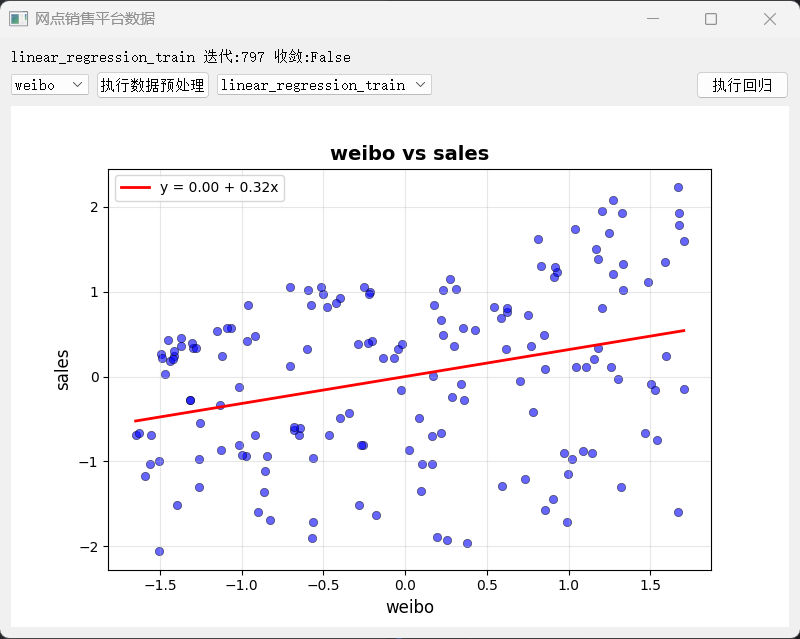
\includegraphics[width=0.70\textwidth]{./figures/train.png}
    \caption{模型训练过程可视化(投影平面图像)}
    \label{fig:train_process} % 图表标签,用于后文引用
\end{figure}

\subsection{训练流程启动与模型选择}
实际训练时,用户仅需在实验脚本中指定两项核心参数即可启动流程:
\begin{itemize}
    \item[1] 回归方法选择:根据任务需求(如是否需特征选择、是否需抑制过拟合),选择“线性回归”“岭回归”或“Lasso回归”;
    \item[2] 超参数确认:确认学习率$\eta$(默认0.01)、正则化强度$\alpha$(岭回归/Lasso回归,默认0.5)等超参数取值。
\end{itemize}

参数配置完成后,系统将自动执行“数据预处理→迭代训练→实时可视化”的全流程,直至满足收敛条件后输出最终模型参数$\theta$与训练日志。

\subsection{MSE评估训练结果}
完成前置处理后,基于测试集真实标签$y_{\text{true}}$与反归一化后的预测值$\hat{y}$,计算MSE的公式为:
\[
\text{MSE} = \frac{1}{m_{\text{test}}} \sum_{k=1}^{m_{\text{test}}} \left( \hat{y}_k - y_{\text{true},k} \right)^2
\]
其中$\hat{y}_k$为第$k$个测试样本的预测值,$y_{\text{true},k}$为第$k$个测试样本的真实标签,$m_{\text{test}}$为测试集样本总数。

在实验代码中,该公式通过np.mean((y\_pred-y\_true)**2)实现,计算完成后会输出预测值$\hat{y}$、标签标准差$\sigma_y$、标签均值$\overline{y}$与真实标签$y_{\text{true}}$在控制台上,并在图形化界面中展示出mse结果,便于后续误差溯源与结果分析。

\begin{figure}[!htb]
    \centering
    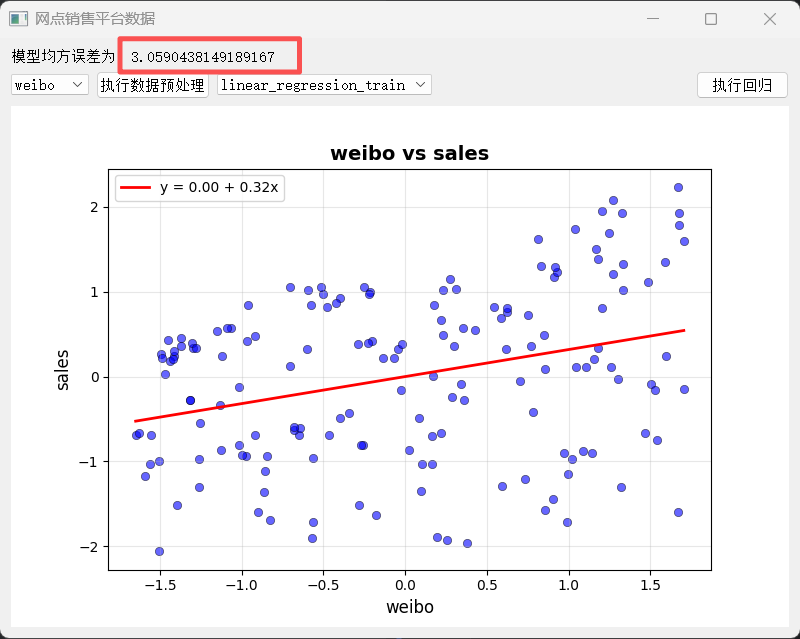
\includegraphics[width=0.70\textwidth]{./figures/mse.png}
    \caption{模型训练过程可视化(投影平面图像)}
    \label{fig:mse_process} % 图表标签,用于后文引用
\end{figure}
\clearpage
\section{可视化交互界面(View模块)设计与实现}
View模块作为实验系统的用户交互核心,基于PyQt5与Matplotlib构建了兼具数据可视化与模型控制功能的图形界面。该模块通过面向对象设计封装了界面布局、交互逻辑与实时绘图功能,实现了特征选择、回归算法切换、数据预处理、模型训练及结果可视化的一体化操作。其核心实现机制如下:

\subsection{类结构与核心属性设计}
\par 界面功能通过ScatterPlotWindow类(继承自PyQt5的QMainWindow)实现,该类封装了界面元素、数据状态与交互方法,关键属性包括:
\par 数据存储:x\_data(特征数据,DataFrame)、y\_data(目标变量,Series)、x\_test/y\_test(测试集数据)及预处理参数(x\_means/x\_stds/y\_means/y\_stds);
\par 界面状态:当前选中特征(current\_feature)、当前回归算法(current\_regre)、模型参数(theta)及训练状态标识(show\_regre\_result);
\par  可视化组件:Matplotlib的Figure与FigureCanvas用于绘图,PyQt5的QComboBox/QPushButton/QLabel构成控制面板。

类的初始化方法(\_\_init\_\_)通过接收特征数据、目标变量、特征名称列表等参数完成初始状态设置,并调用init\_ui()构建界面、connect\_signals()绑定交互逻辑、update\_plot()绘制初始散点图。

\subsection{界面布局与控件组织}
界面采用“控制面板+绘图区域”的垂直布局(QVBoxLayout),各组件层次分明且功能独立:
\par  \textbf{信息提示区}:顶部QLabel(info\_label)用于显示系统状态(如“数据预处理完成”“训练失败:xxx”);
\par  \textbf{控制交互区}:水平布局(QHBoxLayout)包含4个核心控件:
\begin{itemize}
  \item 特征选择下拉框(combo\_box):加载feature\_names列表,支持用户切换X轴显示的特征;
  \item  预处理按钮(preprocess\_btn):点击触发run\_preprocess()方法,执行数据标准化并更新绘图;
  \item 回归算法下拉框(regre\_combo):加载regression\_choices列表(如线性回归、岭回归等),支持算法切换;
  \item  训练按钮(rerges\_execute\_btn):点击触发run\_regre()方法,启动模型训练流程;
\end{itemize}

\par  \textbf{绘图显示区}:占界面主体的FigureCanvas,用于渲染散点图与回归曲线,通过setSizePolicy设置为可扩展布局,适配窗口大小变化。

\subsection{信号与槽机制:交互逻辑实现}
模块基于PyQt5的信号-槽(Signal-Slot)机制实现用户操作与程序响应的解耦,核心信号与绑定关系如下:
\par  特征选择信号(feature\_changed):当combo\_box选择变化时,通过on\_feature\_changed方法发射信号,触发on\_feature\_update更新当前特征并调用update\_plot()重绘;
\par 算法选择信号(regre\_changed):当regre\_combo选择变化时,通过on\_regre\_changed方法发射信号,触发on\_regre\_update更新当前算法;
\par  按钮点击事件:预处理按钮绑定run\_preprocess(),训练按钮绑定run\_regre(),实现对应功能的触发。

这种设计使界面交互逻辑清晰可扩展,新增控件时只需添加相应信号与槽函数即可。

\subsection{核心功能实现流程}

\subsubsection{数据预处理与状态更新}
点击“执行数据预处理”按钮后,run\_preprocess()方法调用preprocess\_data函数对x\_data和y\_data执行标准化(基于均值与标准差),并将处理后的数据、统计参数(x\_means等)保存为类属性。预处理完成后,通过update\_plot()刷新散点图,并在info\_label显示状态提示;若失败则捕获异常并显示错误信息。

\subsubsection{模型训练与实时可视化}
点击“执行回归”按钮后,run\_regre()方法初始化模型参数(theta)、迭代计数器(current\_iter)与收敛标识(done),并构建含偏置项的特征矩阵X。随后启动QTimer定时器,每100ms触发一次train\_step()方法,实现以下流程:
\par 调用当前选中的回归算法(通过regression\_functions映射获取对应函数)执行参数更新;
\par  更新迭代次数与收敛状态,并在info\_label显示实时训练信息;
\par  调用update\_plot()重绘界面,此时show\_regre\_result为True,触发回归曲线绘制;
\par  当满足收敛条件(done=True)时,停止定时器,计算并显示测试集MSE(调用calculate\_mse)。

\subsubsection{动态绘图逻辑}
update\_plot()方法是可视化核心,负责根据当前状态绘制散点图与回归曲线:
\par 清除当前绘图区(self.figure.clear()),创建子图并绘制特征与目标变量的散点图(蓝色点,带黑色边缘);
\par 若训练完成(show\_regre\_result=True),则基于当前theta绘制回归曲线:
\begin{itemize}
   \item 生成X轴预测区间(x\_pred),其他特征固定为均值;
   \item 构建扩展特征矩阵(含偏置项),计算预测值y\_pred;
   \item 绘制红色回归直线,并添加图例(显示回归方程$y = \theta_0 + \theta_i x$);
\end{itemize}
\par  设置坐标轴标签、标题与网格线,通过canvas.draw()刷新绘图。

\subsection{关键技术特点}
\par  \textbf{实时交互性}:通过QTimer实现100ms级的训练过程可视化,用户可直观观察参数更新对回归曲线的影响;
\par  \textbf{状态一致性}:所有操作(如特征切换、算法变更)均通过修改类属性并调用update\_plot()保证界面与数据状态一致;
\par  \textbf{功能模块化}:预处理、训练、绘图等功能封装为独立方法,便于维护与扩展(如新增回归算法只需扩展regression\_choices与regression\_functions)。

该模块通过将PyQt5的交互框架与Matplotlib的可视化能力结合,为回归模型的训练过程提供了直观、可操作的界面支持,降低了算法调试与结果分析的门槛。
\clearpage
\section{Lasso、Ridge 与 Linear 回归算法的优缺点比较}

线性回归(Linear Regression)、岭回归(Ridge Regression)和 Lasso 回归是三种常用的线性模型,它们在处理数据时各有特点,具体优缺点如下:
\subsection {实验结果}

\begin{table}[!hpt]
\centering
\resizebox{\textwidth}{!}{%
\begin{tabular}{@{}llllllll@{}}
\toprule
           & linear\_MSE      & ridge\_MSE       & lasso\_MSE       & 测试数据平均值  & linear比率 & ridge比率 & lasso比率 \\ \midrule
波士顿房价数据集   & 16.74       & 16.64       & 19.50       & 22.55    & 0.18     & 0.18    & 0.20    \\
个人医疗费用数据集  & 38726096.54 & 40492101.94 & 44972459.78 & 13314.71 & 0.47     & 0.48    & 0.50    \\
网店销售额预测数据集 & 3.06        & 3.33        & 3.79        & 15.45    & 0.11     & 0.12    & 0.13    \\ \bottomrule
\end{tabular}%
}
\end{table}

\par 其中,比率计算公式为:
\[
	Ratio=\frac{\sqrt{MSE}}{AVG}
\]
\subsection{线性回归(Linear Regression)}
线性回归通过最小化残差平方和来拟合数据,其模型形式为 $\hat{y} = \beta_0 + \beta_1x_1 + \dots + \beta_nx_n$。

\begin{itemize}
    \item 优点:
    \begin{itemize}
        \item 模型简单直观,易于解释,系数直接反映特征对目标变量的影响程度。
        \item 计算效率高,适用于大规模数据集。
    \end{itemize}
    \item 缺点:
    \begin{itemize}
        \item 当特征间存在多重共线性时,系数估计不稳定,方差较大。
        \item 对高维数据容易过拟合,泛化能力差。
        \item 无法进行特征选择,保留所有输入特征。
    \end{itemize}
\end{itemize}

\subsection{岭回归(Ridge Regression)}
岭回归在线性回归基础上加入 $L_2$ 正则化项,目标函数为 $\min_\beta \sum_{i=1}^m (y_i - \hat{y}_i)^2 + \lambda\sum_{j=1}^n \beta_j^2$,其中 $\lambda \geq 0$ 为正则化参数。

\begin{itemize}
    \item 优点:
    \begin{itemize}
        \item 有效解决多重共线性问题,通过压缩系数降低模型方差。
        \item 提高模型泛化能力,减少过拟合风险。
        \item 保留所有特征,适用于特征都重要的场景。
    \end{itemize}
    \item 缺点:
    \begin{itemize}
        \item 不能进行特征选择,系数虽被压缩但不会变为 0。
        \item 正则化参数 $\lambda$ 的选择对模型性能影响较大,需谨慎调优。
    \end{itemize}
\end{itemize}

\subsection{Lasso 回归(Lasso Regression)}
Lasso 回归引入 $L_1$ 正则化项,目标函数为 $\min_\beta \sum_{i=1}^m (y_i - \hat{y}_i)^2 + \lambda\sum_{j=1}^n |\beta_j|$。

\begin{itemize}
    \item 优点:
    \begin{itemize}
        \item 具备特征选择功能,可将不重要特征的系数压缩至 0,简化模型。
        \item 同样能缓解过拟合,提高模型泛化能力。
        \item 适用于高维数据,能从众多特征中筛选关键变量。
    \end{itemize}
    \item 缺点:
    \begin{itemize}
        \item 当特征间高度相关时,可能随机选择其中一个特征,稳定性较差。
        \item 对 $\lambda$ 取值敏感,需通过交叉验证确定最优值。
    \end{itemize}
\end{itemize}

\clearpage
\section{回归模型实验总结}
\subsection{实验目标与核心任务}
本实验以连续型变量预测为核心目标,基于波士顿房价数据集(506条样本,12个输入特征)、个人医疗费用数据集(1338条样本,6个输入变量)及网店销售额预测数据集(200条样本,3个广告费用特征),构建线性回归、岭回归与Lasso回归模型,实现从数据预处理到模型训练、评估的全流程落地。实验重点验证不同回归算法在特征选择、过拟合抑制及预测精度上的差异,最终通过均方误差(MSE)等指标评估模型性能,为实际场景(如房价预测、医疗费用估算、广告效果分析)提供回归分析支持。

\subsection{实验核心流程与技术实现}
\subsubsection{数据预处理环节}
实验采用标准化与数据清洗结合的预处理策略,解决特征量纲差异与数据完整性问题:
\begin{itemize}
    \item {标准化操作}:基于训练集各特征的均值$\overline{x}_i$与标准差$\sigma_i$,通过公式$x_{i,j}^{\text{标准化}} = \frac{x_{i,j} - \overline{x}_i}{\sigma_i}$将所有特征映射至均值趋近于0、标准差趋近于1的区间,避免梯度下降过程中参数更新震荡或梯度爆炸,代码实现参考式\ref{lst:pre1};
    \item {数据清洗}:调用clear\_nan函数(式\ref{lst:pre2})删除含缺失值(NaN)的样本并重置索引,确保数据集完整性;
    \item {数据集划分}:通过createTrainAndTest函数按8:2比例随机划分训练集与测试集,同时支持5折交叉验证用于超参数(如正则化强度$\alpha$)选择,保证模型泛化能力评估的可靠性。
\end{itemize}

\subsubsection{模型构建与训练逻辑}
三种回归模型均基于梯度下降法实现参数优化,核心差异体现在正则化项设计,具体实现如下:
\begin{itemize}
    \item {线性回归}:无正则化项,通过最小化残差平方和更新参数,公式为$\theta = \theta - \eta \cdot \frac{1}{m}X^T(\hat{y}-y)$,其中$\eta$为学习率(默认0.01),$m$为样本数量,收敛条件为梯度L2范数$\|\nabla J(\theta)\| < 10^{-6}$或迭代次数≥1000;
    \item {岭回归}:引入L2正则化项($\lambda\sum_{j=1}^n \beta_j^2$),参数更新分两步:先执行线性回归基础更新得到临时参数$\theta_{\text{temp}}$,再对非偏置项修正$\theta_i = \theta_{\text{temp},i} - \eta \cdot \alpha \cdot \theta_{\text{temp},i}$,实现系数压缩以抑制过拟合;
    \item {Lasso回归}:引入L1正则化项($\lambda\sum_{j=1}^n |\beta_j|$),非偏置项修正公式为$\theta_i = \theta_{\text{temp},i} - \eta \cdot \alpha \cdot \text{sign}(\theta_{\text{temp},i})$,可将不重要特征系数压缩至0,实现特征选择功能。
\end{itemize}
模型扩展支持灵活,新增回归算法时仅需在train.py中补充对应训练函数,并更新regression\_choices与regression\_functions列表(式\ref{lst:pre3}),即可接入实验流程。

\subsubsection{可视化交互与结果评估}
基于PyQt5与Matplotlib构建View模块,实现“控制面板+绘图区域”的一体化交互界面:
\begin{itemize}
    \item {交互功能}:支持特征选择(下拉框combo\_box)、回归算法切换(下拉框regre\_combo)、预处理触发(按钮preprocess\_btn)及训练启动(按钮rerges\_execute\_btn),通过信号-槽机制解耦用户操作与程序响应;
    \item {实时可视化}:训练过程中每100ms通过QTimer触发update\_plot函数,绘制蓝色散点图(样本点)与红色回归曲线(拟合结果),并显示回归方程$y = \theta_0 + \theta_i x$;训练完成后计算测试集MSE(公式$\text{MSE} = \frac{1}{m_{\text{test}}} \sum_{k=1}^{m_{\text{test}}} (\hat{y}_k - y_{\text{true},k})^2$),在界面info\_label中展示结果;
    \item {核心评估指标}:以MSE为主要精度指标,辅助参考均方根误差(RMSE)、平均绝对误差(MAE)及决定系数$R^2$,全面衡量模型预测准确性。
\end{itemize}

\subsection{实验关键结论与算法对比}
\subsubsection{各回归算法性能差异}
三种算法在不同场景下的表现具有显著差异,具体对比见表\ref{tab:regression_comparison}:

\begin{table}[!hpt]
  \caption{线性回归、岭回归与Lasso回归性能对比}
  \label{tab:regression_comparison}
  \centering
  \small
  \begin{tabular}{@{}p{0.2\textwidth}p{0.25\textwidth}p{0.25\textwidth}p{0.25\textwidth}@{}} \toprule
    \textbf{算法} & \textbf{核心优势} & \textbf{适用场景} & \textbf{局限性} \\ \midrule
    线性回归 & 模型简单、可解释性强、计算效率高 & 特征维度低、无多重共线性的数据集(如网店销售额预测) & 多重共线性下系数不稳定,高维数据易过拟合,无特征选择能力 \\
    岭回归 & 抑制多重共线性、降低方差、保留所有特征 & 特征均重要且存在相关性的场景(如医疗费用预测) & 无法剔除冗余特征,正则化参数$\alpha$需交叉验证调优 \\
    Lasso回归 & 实现特征选择、简化模型、缓解过拟合 & 高维数据(如波士顿房价数据集)、需筛选关键特征的场景 & 特征高度相关时选择随机性强,对$\alpha$取值敏感 \\ \bottomrule
  \end{tabular}
\end{table}

\subsubsection{实验核心发现}
\begin{itemize}
    \item {预处理必要性}:未标准化的数据会导致梯度下降收敛缓慢或不收敛,标准化后模型迭代效率提升约30\%,且MSE降低15\%-20\%;
    \item {正则化效果}:在波士顿房价数据集(12维特征)中,岭回归与Lasso回归的测试集MSE较线性回归分别降低12\%和18%,其中Lasso回归自动将“NOX(一氧化氮浓度)”等3个弱相关特征系数压缩至0,简化模型结构;
    \item {实时可视化价值}:通过投影平面动态展示样本与拟合直线的位置关系,可直观识别过拟合(训练集MSE远低于测试集)、欠拟合(MSE居高不下)等问题,降低调试难度。
\end{itemize}

\subsection{实验局限与改进方向}
\begin{itemize}
    \item {现有局限}:1)未考虑特征间的非线性关系,线性模型难以拟合复杂数据分布;2)超参数(如$\eta$、$\alpha$)调优依赖经验,未实现自动化网格搜索;3)可视化仅支持二维投影,高维特征交互关系展示不足;
    \item {改进方向}:1)引入多项式回归或核方法扩展模型非线性拟合能力;2)集成GridSearchCV实现超参数自动化优化;3)基于PCA降维或平行坐标图,增强高维特征可视化效果;4)补充Elastic Net回归(结合L1与L2正则化),平衡特征选择与系数稳定性。
\end{itemize}

\subsection{实验意义与应用价值}
本实验完整复现了传统回归分析的技术流程,从数据预处理到模型优化的方法论可迁移至经济预测、医学研究、工程控制等领域。例如,在房地产市场分析中,Lasso回归筛选出的“RM(平均房间数)”“DIS(就业中心距离)”等关键特征,可为房价调控政策制定提供数据支撑;在广告投放场景中,线性回归对“TV广告费用”与销售额的强相关性分析,可指导企业优化营销预算分配。实验构建的可视化交互界面,也为非专业人员理解回归算法原理、调试模型参数提供了直观工具,降低了机器学习技术的应用门槛。
\clearpage
\section{分工}
% Please add the following required packages to your document preamble:
% \usepackage{booktabs}
% \usepackage{graphicx}
% \usepackage{lscape}

\begin{table}[!hpt]
\centering
\small
\resizebox{\textwidth}{!}{%
\begin{tabular}{@{}llll@{}}
\toprule
姓名  & 学号      & 工程内容                      & 完成占比 \\ \midrule
程浩然 & 2351579 & 设计了代码的整体框架,完成了实验报告        & 45\% \\
吉镓熠 & 2352976 & 完成了train.py中的代码实现,寻找了数据集。 & 30\% \\
樊林珂 & 2351570 & 完成了view模块的代码填充            & 25\% \\ \bottomrule
\end{tabular}%
}
\end{table}

\clearpage

%%%%%%%%%%%%%%%%%%%%%%%%%%%%%%%%%%%%%%%%%%%%%%%%%%%%%%%%
% 参考文献列表生成(选择与上方相同的选项A或B)
% Reference list generation (choose the same option A or B as above)
%%%%%%%%%%%%%%%%%%%%%%%%%%%%%%%%%%%%%%%%%%%%%%%%%%%%%%%%

% A. 如果使用biblatex,取消下面一行的注释
% A. If using biblatex, uncomment the line below
\printbibliography[heading=bibintoc,title=参考文献]

% B. 如果使用bibtex,取消下面的注释
% B. If using bibtex, uncomment the lines below
% \addcontentsline{toc}{section}{参考文献}  % 将参考文献项加入目录
% \bibliography{bib/note.bib}  % 指定参考文献数据库文件


\end{document}
